\subsection{Теоретический минимум к кр 1}


\begin{enumerate}
	\item Классическое определение вероятности
	\item Определение условной вероятности
	\item Определение независимости случайных событий
	\item Формула полной вероятности
	\item Формула Байеса
	\item Функция распределения случайной величины. Определение и свойства.
	\item Функция плотности. Определение и свойства.
	\item Математическое ожидание. Определения для дискретного и абсолютно непрерывного случаев. Свойства.
	\item Дисперсия. Определение и свойства.
	\item Законы распределений. Определение, $\E(X)$, $\Var(X)$:
	\begin{enumerate}
	\item Биномиальное распределение
	\item Распределение Пуассона
	\item Геометрическое распределение
	\item Равномерное распределение
	\item Экспоненциальное распределение
	\end{enumerate}
\end{enumerate}


\subsection{Задачный минимум к кр 1}

\begin{enumerate}
\item  Пусть $\P(A) = 0.3, \P(B) = 0.4, \P(A\cap B) = 0.1 $. Найдите
	\begin{enumerate}
		\item  $\P(A|B)$
		\item  $\P(A\cup B)$
		\item  Являются ли события $A$ и $B$ независимыми?
	\end{enumerate}



\item  Пусть $\P(A) = 0.5, \P(B) = 0.5, \P(A\cap B) = 0.25 $. Найдите
\begin{enumerate}
	\item  $\P(A|B)$
	\item  $\P(A\cup B)$
	\item  Являются ли события $A$ и $B$ независимыми?
\end{enumerate}



\item  Карлсон выложил кубиками слово КОМБИНАТОРИКА. Малыш выбирает наугад четыре кубика и выкладывает их в случайном порядке.
Найдите вероятность того, что при этом получится слово КОРТ.


\item  Карлсон выложил кубиками слово КОМБИНАТОРИКА. Малыш выбирает наугад четыре кубика и выкладывает их в случайном порядке.
Найдите вероятность того, что при этом получится слово РОТА.

\item  В первой урне 7 белых и 3 черных шара, во второй урне 8 белых и 4 черных
шара, в третьей урне 2 белых и 13 черных шаров. Из этих урн наугад выбирается одна урна. Какова вероятность того, что шар, взятый наугад из выбранной урны, окажется белым?


\item  В первой урне 7 белых и 3 черных шара, во второй урне 8 белых и 4 черных
шара, в третьей урне 2 белых и 13 черных шаров. Из этих урн наугад выбирается одна урна. Какова вероятность того, что была выбрана первая урна, если шар, взятый наугад из выбранной урны, оказался белым?


\item  В операционном отделе банка работает 80\% опытных сотрудников и 20\%
неопытных. Вероятность совершения ошибки при очередной банковской операции
опытным сотрудником равна 0.01, а неопытным — 0.1. Найдите вероятность совершения ошибки при очередной банковской операции в этом отделе.


\item  В операционном отделе банка работает 80\% опытных сотрудников и 20\%
неопытных. Вероятность совершения ошибки при очередной банковской операции
опытным сотрудником равна 0.01, а неопытным — 0.1. Известно, что при очередной банковской операции была допущена ошибка. Найдите вероятность того, что ошибку допустил неопытный сотрудник.

\item  Пусть случайная величина $X$ имеет таблицу распределения:

\begin{tabular}{ ll l l}
	\toprule
	$X$ & -1  & 0  & 1 \\
	$\P_X$ & 0.25  & c  & 0.25 \\
  \bottomrule
\end{tabular}

Найдите
	\begin{enumerate}
	\item константу $c$
	\item $\P(\{X \geq 0\})$
	\item $\P(\{X < -3\}])$
	\item $\P(\{X \in [-\frac{1}{2}; \frac{1}{2}]\})$
	\item функцию распределения случайной величины $X$
	\item имеет ли случайная величина $X$ плотность распределения?
	\end{enumerate}


\item  Пусть случайная величина $X$ имеет таблицу распределения:

\begin{tabular}{ llll}
\toprule
$X$ & -1  & 0  & 1 \\
$\P_X$ & 0.25  & c  & 0.25 \\
\bottomrule
\end{tabular}

Найдите
\begin{enumerate}
	\item константу $c$
	\item $\E(X)$
	\item $\E(X^2)$
	\item $\Var(X)$
	\item $\E(|X|)$
\end{enumerate}

\item  Пусть случайная величина $X$ имеет таблицу распределения:

\begin{tabular}{ lll l}
\toprule
$X$ & -1  & 0  & 1 \\
$\P_X$ & 0.25  & c  & 0.5 \\
\bottomrule
\end{tabular}

Найдите
	\begin{enumerate}
	\item константу $c$
	\item $\P(\{X \geq 0\})$
	\item $\P(\{X < -3\}])$
	\item $\P(\{X \in [-\frac{1}{2}; \frac{1}{2}]\})$
	\item функцию распределения случайной величины $X$
	\item имеет ли случайная величина $X$ плотность распределения?
\end{enumerate}

\item  Пусть случайная величина $X$ имеет таблицу распределения:

\begin{tabular}{ l l l l}
  \toprule
$X$ & -1  & 0  & 1 \\
$\P_X$ & 0.25  & c  & 0.5 \\
\bottomrule
\end{tabular}

Найдите
\begin{enumerate}
	\item константу $c$
	\item $\E(X)$
	\item $\E(X^2)$
	\item $\Var(X)$
	\item $\E(|X|)$
\end{enumerate}

\item Пусть случайная величина $X$ имеет биномиальное распределение с
параметрами $n = 4$ и $\P = \frac{3}{4}$.
 Найдите
\begin{enumerate}
	\item $\P(\{X = 0\})$
	\item $\P(\{X > 0\})$
	\item $\P(\{X < 0\})$
	\item $\E(X)$
	\item $\Var(X)$
	\item  наиболее вероятное значение, которое принимает случайная величина $X$
\end{enumerate}

\item Пусть случайная величина $X$ имеет биномиальное распределение с
параметрами $n = 5$ и $\P = \frac{2}{5}$.
Найдите
\begin{enumerate}
	\item $\P(\{X = 0\})$
	\item $\P(\{X > 0\})$
	\item $\P(\{X < 0\})$
	\item $\E(X)$
	\item $\Var(X)$
	\item  наиболее вероятное значение, которое принимает случайная величина $X$
\end{enumerate}


\item  Пусть случайная величина X имеет распределение Пуассона с параметром $\lambda = 100$ . Найдите
\begin{enumerate}
	\item $\P(\{X = 0\})$
	\item $\P(\{X > 0\})$
	\item $\P(\{X < 0\})$
	\item $\E(X)$
	\item $\Var(X)$
	\item  наиболее вероятное значение, которое принимает случайная величина $X$
\end{enumerate}


\item  Пусть случайная величина X имеет распределение Пуассона с параметром $\lambda = 101$ . Найдите
\begin{enumerate}
	\item $\P(\{X = 0\})$
	\item $\P(\{X > 0\})$
	\item $\P(\{X < 0\})$
	\item $\E(X)$
	\item $\Var(X)$
	\item  наиболее вероятное значение, которое принимает случайная величина $X$
\end{enumerate}


\item В лифт 10-этажного дома на первом этаже вошли 5 человек. Вычислите
вероятность того, что на 6-м этаже выйдет хотя бы один человек.


\item В лифт 10-этажного дома на первом этаже вошли 5 человек. Вычислите
вероятность того, что на 6-м этаже не выйдет ни один человек.


\item При работе некоторого устройства время от времени возникают сбои.
Количество сбоев за сутки имеет распределение Пуассона. Среднее количество сбоев за сутки равно 3. Найти вероятность того, что в течение суток произойдет хотя бы один сбой.


\item При работе некоторого устройства время от времени возникают сбои.
Количество сбоев за сутки имеет распределение Пуассона. Среднее количество сбоев за сутки равно 3. Найти вероятность того, что за двое суток не произойдет ни одного сбоя.


\item Пусть случайная величина $X$ имеет плотность распределения

\[
f_X(x) =
	\begin{cases}
	c,\text{ при }  x \in [-1; 1] \\
	0,\text{ при } x \notin  [-1; 1] \\
	\end{cases}
\]

Найдите
\begin{enumerate}
	\item константу $c$
	\item $\P(\{X \leq 0\})$
	\item $\P(\{X \in [\frac{1}{2}; \frac{3}{2}]\})$
	\item $\P(\{X \in [2;3]\}$
	\item $F_X(x)$
\end{enumerate}


\item Пусть случайная величина $X$ имеет плотность распределения

\[
f_X(x) =
	\begin{cases}
	c,\text{ при }  x \in [-1; 1] \\
	0,\text{ при } x \notin  [-1; 1] \\
	\end{cases}
\]

Найдите
\begin{enumerate}
	\item константу $c$
	\item $\E(X)$
	\item $\E(X^2)$
	\item $\Var(X)$
	\item $\E(|X|)$
\end{enumerate}


\item Пусть случайная величина $X$ имеет плотность распределения

\[
f_X(x) =
	\begin{cases}
	cx,\text{ при }  x \in [0; 1] \\
	0,\text{ при } x \notin  [0; 1] \\
	\end{cases}
\]

Найдите
\begin{enumerate}
	\item константу $c$
	\item $\P(\{X \leq \frac{1}{2}\})$
	\item $\P(\{X \in [\frac{1}{2}; \frac{3}{2}]\})$
	\item $\P(\{X \in [2;3]\}$
	\item $F_X(x)$
\end{enumerate}


\item Пусть случайная величина $X$ имеет плотность распределения

\[
f_X(x) =
	\begin{cases}
	cx,\text{ при }  x \in [0; 1] \\
	0,\text{ при } x \notin  [0; 1] \\
	\end{cases}
\]

Найдите
\begin{enumerate}
	\item константу $c$
	\item $\E(X)$
	\item $\E(X^2)$
	\item $\Var(X)$
	\item $\E(\sqrt{X})$
\end{enumerate}
\end{enumerate}



\subsubsection*{Ответы}

\begin{enumerate}
	\item
			\begin{enumerate}
				\item 0.25
				\item 0.6
				\item нет
			\end{enumerate}
	\item
			\begin{enumerate}
				\item 0.5
				\item  0.75
				\item нет
			\end{enumerate}
	\item $\frac{4}{10 \cdot 11 \cdot 12 \cdot 13}$
	\item $\frac{4}{10 \cdot 11 \cdot 12 \cdot 13}$
	\item 0.5


	\item 0.42
	\item 0.028
	\item $\frac{5}{7}$
	\item
			\begin{enumerate}
				\item 0.5
				\item 0.75
				\item 0
				\item 0.5
			\end{enumerate}
	\item
			\begin{enumerate}
				\item 0.5
				\item  0
				\item  0.5
				\item  0.5
				\item  0.5
			\end{enumerate}
	\item
			\begin{enumerate}
				\item 0.25
				\item 0.75
				\item 0
				\item 0.5
			\end{enumerate}
	\item
			\begin{enumerate}
				\item 0.25
				\item 0.25
				\item 0.75
				\item 0.5
				\item 0.75
			\end{enumerate}
	\item
			\begin{enumerate}
				\item $\left( \frac{1}{4} \right) ^4$
				\item $1 - \left( \frac{1}{4} \right) ^4$
				\item 0
				\item 3
				\item 0.75
				\item 2, 3
			\end{enumerate}
	\item
			\begin{enumerate}
				\item $\left( \frac{3}{5} \right) ^5$
				\item $1 - \left( \frac{3}{5} \right) ^5$
				\item 0
				\item 2
				\item 1.2
				\item 2
			\end{enumerate}
	\item
			\begin{enumerate}
				\item $e^{-100}$
				\item $1 - e^{-100}$
				\item 0
				\item 100
				\item 100
			\end{enumerate}
	\item
			\begin{enumerate}
				\item $e^{-101}$
				\item $1 - e^{-101}$
				\item 0
				\item 101
				\item 101
			\end{enumerate}
	\item $1 - \frac{8^5}{9^5}$
	\item $\frac{8^5}{9^5}$
	\item $1 - e^{-3}$
	\item $e^{-3}$
	\item
			\begin{enumerate}
				\item 0.5
				\item 0.25
				\item 0.125
				\item 1
			\end{enumerate}
	\item
			\begin{enumerate}
				\item 0.5
				\item 0.5
				\item $\frac{1}{3}$
				\item $\frac{1}{12}$
				\item 1
			\end{enumerate}
	\item
			\begin{enumerate}
				\item 2
				\item 0.25
				\item $\frac{3}{4}$
				\item 1
			\end{enumerate}
	\item
			\begin{enumerate}
				\item 2
				\item 0.5
				\item 0.5
				\item 0
				\item 0.8
			\end{enumerate}
\end{enumerate}




\subsection{Контрольная работа 1, базовый поток, 24.10.2017}

\subsubsection*{Минимум}

\begin{enumerate}
\item Функция распределения случайной величины: определения и свойства.
\item Экспоненциальное распределение: определение, математическое ожидание и дисперсия.
\item В операционном отделе банка работает 80\% опытных сотрудников и 20\% неопытных. Вероятность совершения ошибки при очередной банковской операции опытным сотрудником равна $0.01$, а неопытным — $0.1$. Известно, что при очередной банковской операции была допущена ошибка. Найдите вероятность того, что ошибку допустил неопытный сотрудник.
\item При работе некоторого устройства время от времени возникают сбои. Количество сбоев за сутки имеет распределение Пуассона. Среднее количество сбоев за сутки равно 3. Найдите вероятность того, что за двое суток не произойдет ни одного сбоя.

\end{enumerate}

\subsubsection*{Задачи}

\begin{enumerate}

\item Правильный кубик подбрасывают один раз. Событие $A$ — выпало чётное число, событие $B$ — выпало число кратное трём, событие $C$ — выпало число, большее трёх.

\begin{enumerate}
\item Сформулируйте определение независимости двух событий;
\item Определите, какие из пар событий $A$, $B$ и $C$ будут независимыми.
\end{enumerate}


\item Теоретический минимум (ТМ) состоит из 10 вопросов, задачный (ЗМ) — из 24 задач.
Каждый вариант контрольной содержит два вопроса из ТМ и две задачи из ЗМ.
Чтобы получить за контрольную работу оценку 4 и выше, необходимо и достаточно правильно ответить на каждый вопрос ТМ и задачу ЗМ доставшегося варианта. Студент Вася принципиально выучил только $k$ вопросов ТМ и две трети ЗМ.
\begin{enumerate}
\item Сколько всего можно составить вариантов, отличающихся хотя бы одним заданием в ТМ или ЗМ части? Порядок заданий внутри варианта не важен.
\item Найдите вероятность того, что Вася правильно решит задачи ЗМ;
\item Дополнительно известно, что Васина вероятность правильно ответить на вопросы ТМ, составляет $1/15$. Сколько вопросов ТМ выучил Вася?
\end{enumerate}

\item Производитель молочных продуктов выпустил новый низкокалорийный йогурт Fit и утверждает, что он вкуснее его более калорийного аналога Fat.
Четырем независимым экспертам предлагают выбрать наиболее вкусный йогурт из трёх, предлагая им в одинаковых стаканчиках в случайном порядке два Fat и один Fit.
Предположим, что йогурты одинаково привлекательны.
Величина $\xi$ — число экспертов, отдавших предпочтение Fit.
\begin{enumerate}
\item Какова вероятность, что большинство экспертов выберут Fit?
\item Постройте функцию распределения величины $\xi$;
\item Каково наиболее вероятное число экспертов, отдавших предпочтение йогорту Fit?
\item Вычислите математическое ожидание и дисперсию $\xi$.
\end{enumerate}

\item Дядя Фёдор каждую субботу закупает в магазине продукты по списку, составленному котом Матроскином. Список не изменяется, и в него всегда входит 1 кг сметаны, цена которого является равномерно распределённой величиной $\alpha$, принимающей значения от 250 до 1000 рублей. Стоимость остальных продуктов из списка в тысячах рублей является случайной величиной $\xi$ с функцией распределения

\[
F(x)=\begin{cases}
1-\exp(-x^2 ), \text{ если } x \geq 0 \\
0, \text{ иначе.}\\
\end{cases}
\]

\begin{enumerate}
\item Какую сумму должен выделить кот Матроскин дяде Фёдору, чтобы её достоверно хватало на покупку сметаны?
\item Какую сумму должен выделить кот Матроскин дяде Фёдору, чтобы Дядя Фёдор с вероятностью 0.9 мог оплатить продукты без сметаны?
\item Найдите математическое ожидание стоимости продуктов без сметаны;
\item Найдите математическое ожидание стоимости всего списка.
\item Какова вероятность того, что общие расходы будут в точности равны их математическому ожиданию?
\end{enumerate}

Подсказка: $\int_0^{\infty} \exp(-x^2) \, dx = \sqrt{\pi} / 2$.

\item Эксперт с помощью детектора лжи пытается определить, говорит ли подозреваемый правду. Если подозреваемый говорит правду, то эксперт ошибочно выявляет ложь с вероятностью 0.1. Если подозреваемый обманывает, то эксперт выявляет ложь с вероятностью 0.95.

В деле об одиночном нападении подозревают десять человек, один из которых виновен и будет лгать, остальные невиновны и говорят правду.

\begin{enumerate}
\item Какова вероятность того, что детектор покажет, что конкретный подозреваемый лжёт?
\item Какова вероятность того, что подозреваемый невиновен, если детектор показал, что он лжёт?
\item Какова вероятность того, что эксперт точно выявит преступника?
\item Какова вероятность того, что эксперт ошибочно выявит  преступника, то есть покажет, что лжёт невиновный, а все остальные говорят правду?
\end{enumerate}



\end{enumerate}


\subsection{Контрольная работа 1, базовый поток, 24.10.2017, решения}

\begin{enumerate}
\item
\begin{enumerate}
\item События называются независимыми, если  $ \P(A \cap B) = \P(A) \cdot \P(B)$
\item Запасёмся всеми нужными вероятностями:

$\P(A) = \frac{1}{2}$

$\P(B) = \frac{1}{3}$

$\P(C) = \frac{1}{2}$

$\P(A \cap C) = \frac{1}{3} $ — выпадет чётое число больше трёх

$\P(A \cap B)  = \frac{1}{6}$ — выпадет чётное число, кратное трём

$\P(A \cap C) = \frac{1}{6}$ — выпадет число, большее трёх и кратное трём

Теперь можно проверять независимость:

$\P(A \cap C) \neq \P(A) \cdot \P(C) \Rightarrow$  не являются независимыми

$ \P(A \cap B) = \P(A) \cdot \P(B) \Rightarrow$ являются независимыми

$ \P(B \cap C) = \P(B) \cdot \P(C) \Rightarrow$ являются независимыми

\end{enumerate}
\item
\begin{enumerate}
\item Количество возможных вариантов ТМ: $ C_{10}^2 $,  количество возможных вариантов ЗМ: $ C_{24}^2 $. Количество их возможных сочетаний: $ C_{10}^2 \cdot C_{24}^2$ , где $ C_n^k = \frac{n!}{k!(n-k)!}$.
\item По классическому определению вероятностей, предполагая исходы равновероятными, искомая вероятность равна $ \frac{C_{16}^2}{C_{24}^2} $
\item По тому же принципу:
\[
\frac{C_k^2}{C_{10}^2} = \frac{1}{15} \Rightarrow \frac{\frac{k!}{2!(k-2)!}}{\frac{10!}{2! \cdot 8!}} = \frac{1}{15} \Rightarrow \frac{(k-1)k}{2}\frac{ 2}{9 \cdot 10} = \frac{1}{15}
\]
Получаем квадратное уравнение вида $ k^2 - k - 6 = 0 $ с корнями $-2$ и $3$. Так как $k$ не может быть отрицательным, ответ $3$.
\end{enumerate}
\item
\begin{enumerate}
\item Если эксперт отдаёт предпочтение Fit, то это можно интерпретировать как «успех» в схеме Бернулли. Так как $\xi$ - количество успехов, $ k \in [0;4]$, $p = \frac{1}{3} $, то
\[
\P(\xi = k) = C_n^k(p)^k(1-p)^{n-k}
\]

Большинство означает, что либо три, либо четыре эксперта выбрали Fit.
\[
\P(\xi = 3) = C_4^3\left(\frac{1}{3}\right)^3 \left(\frac{2}{3}\right)^{1} = \frac{8}{81}
\]
\[
\P(\xi = 4) = C_4^4\left(\frac{1}{3}\right)^4 \left(\frac{2}{3}\right)^{0} = \frac{1}{81}
\]
\[
\P( \xi > 2) =  \frac{9}{81}
\]
\item Аналогично:

\[ \P(\xi = 0) = C_4^0\left(\frac{1}{3}\right)^0 \left(\frac{2}{3}\right)^{4} = \frac{16}{81}\]

\[ \P(\xi = 1) = C_4^1\left(\frac{1}{3}\right)^1 \left(\frac{2}{3}\right)^{3} = \frac{32}{81}\]

\[ \P(\xi = 2) = C_4^2\left(\frac{1}{3}\right)^2 \left(\frac{2}{3}\right)^{2} = \frac{24}{81}\]

\begin{figure}[h!]
    \noindent\centering{
    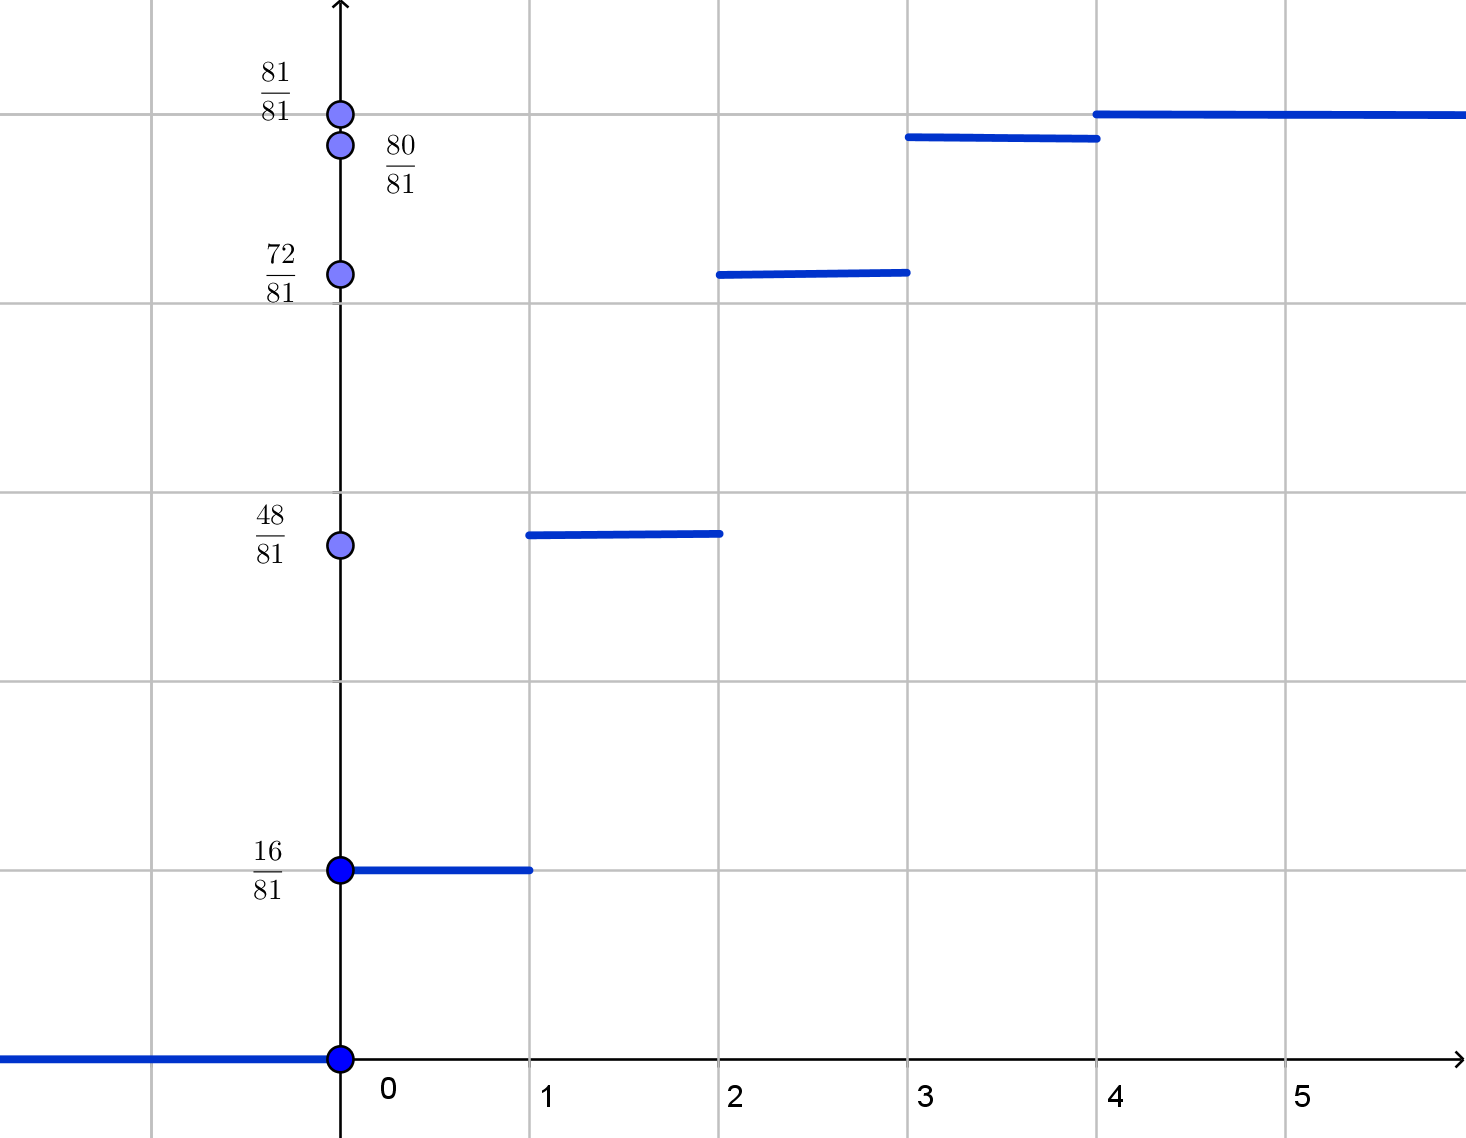
\includegraphics[width=80mm]{images/kr1_2017_3.png}
    }
    \caption{Функция распределения}
    \label{cdf_kr2017}
\end{figure}

\item Все вероятности посчитаны, видим, что наибольшая достигается при $\xi=1$.
\item $\E(X) = np = \frac{4}{3} $, $ \Var(X) = npq = \frac{8}{9}$
\end{enumerate}
\item
\begin{enumerate}
\item Так как указано, что цена сметаны распределена равномерно на отерзке $[250, 1000]$, максимальное значение цены — $1000$, это и есть необходимая сумма.
\item Вспомним, что функция распределения $F(x) = \P(X \leq x)$, нужно найти такой $x$, что $ \P(X \leq x)=0.9$:
\[
0.9 = 1 - \exp({-x^{2}}) \Rightarrow \exp(-x^{2}) = 0.1 \Rightarrow -x^2 = \ln(0.1)  \Rightarrow x=  \sqrt{-\ln(0.1)}
\]
\item Взяв производную от функции распределения списка без сметаны, получим функцию плотности:
\[
f_X(x) =
\begin{cases}
2x\exp(-x^2) & x \ge 0 \\
0 & \text{иначе}
\end{cases}
\]
Найдём математическое ожидание:
\[
\int_{0}^{+\infty}2x^2\exp({-x^2}) dx = -x \exp({-x^2})\big|_0^{+\infty} + \int_{0}^{+\infty}\exp({-x^2}) dx = \frac{\sqrt{\pi}}{2}
\]
\item Математическое ожидание суммы случайных величин равно сумме математических ожиданий случайных влечин, если они существуют. Математическое ожидание от цены сметаны равно: $ \frac{1000 + 250}{2} = 625 $
Математическое ожидание списка без сметаны было найдено в предыдущем пункте, его осталось перевести в рубли. Получаем ответ: $ 625 + \frac{\sqrt{\pi}}{2} \cdot 1000 $.
\item Так как обе величины имеют абсолютно непрерывные распределения, вероятность попасть в конкретную точку равна нулю.
\end{enumerate}
\item
\begin{enumerate}
\item $\P(\text{детектор показл ложь и подозреваемый лжёт}) = 0.9 \cdot 0.1 + 0.1 \cdot 0.95 = 0.185$
\item $\P(\text{невниовен}|\text{детектор показал ложь}) = \frac{0.9\cdot0.1}{0.185} = \frac{90}{185}$
\item $\P(\text{эксперт точно выявит преступника}) = (0.9)^9 \cdot 0.95$
\item $\P(\text{эксперт ошибочно выявит преступника}) = 9 \cdot 0.1 \cdot 0.9^8\cdot 0.05$
\end{enumerate}


%\item
%$\P(Ложь|Лжёт) = 0.95 $

%$\P(Ложь|Не лжёт) = 0.1 $

%$\P({Лжёт}) = \frac{1}{10} $

%\P(\text{Не лжёт}) = \dfrac{9}{10} $

%\begin{enumerate}
%	\item
%	По формуле полной вероятности: \[  \P(Ложь) = 0.95 \cdot 0.1 + 0.1 \cdot 0.9 = 0.185 \]
%	\item
%	По формуле Байеса: \[ \P(\text{Не лжёт}|Ложь) = \dfrac{0.1 \cdot 0.9}{0.185} = 0.486\]
%    \item
%    Событие "эксперт точно выявит преступника" соответствует событию "эксперт выявит, что лгун лжет, и      что остальные говорят правду".  Таким образом:  \[ \P = 0.1 \cdot 0.95 + 0.9 \cdot 0.9  = 0.905\]
%    \item
%    Это означает, что эксперт выберет 8 человек из 9 невиновных и скажет, что они говорят правду
%    (количество вариантов выбрать так людей  $С_9^8$ ), а также выберет 1 виновного и скажет, что он
%    говорит правду (количество вариантов это сделать 1), и выберет одного невиновного и скажет, что он
%    лжет (количество вариантов выбрать так человека $С_9^1$ ). Просуммируем все с учетом вероятностей,
%    указанных в условии: \[ \P = с_9^8 \cdot 0.9 \cdot 0.9 \cdot C_9^1 \cdot 0.9 \cdot 0.1 \cdot 1 \cdot 0.1
%    \cdot 0.05 = 0. 26244\]

%\end{enumerate}
\end{enumerate}



\subsection{Контрольная работа 1, ИП, 24.10.2017}


Ровно 272 года назад императрица Елизавета повелела завезти во дворцы котов для ловли мышей.


\begin{enumerate}

\item В отсутствии кота Леопольда мыши Белый и Серый подкидывают по очереди игральный додекаэдр
%\footnote{Леопольд подсказывает по случаю праздника, что у додекаэдра 12 граней :)}
.
Сыр достаётся тому, кто первым выкинет число 6. Начинает подкидывать Белый.

\begin{enumerate}
  \item Какова вероятность того, что сыр достанется Белому?
  \item Сколько в среднем бросков продолжается игра?
  \item Какова дисперсия числа бросков?
\end{enumerate}

\item Микки Маус, Белый и Серый решили устроить труэль из любви к мышки Мии. Сначала стреляет Микки, затем Белый, затем Серый, затем снова Микки и так до тех пор, пока в живых не останется только один.

Прошлые данные говорят о том, что Микки попадает с вероятностью $1/3$, Белый — с вероятностью $2/3$, а Серый стреляет без промаха.

Найдите оптимальную стратегию каждого мыша.

\item Микки Маус, Белый и Серый пойманый злобным котом Леопольдом до начала труэли. И теперь Леопольд будет играть с ними в странную игру.

В комнате три закрытых внешне неотличимых коробки: с золотом, серебром и платиной. Общаться после начала игры мыши не могут, но могут заранее договориться о стратегии.

Правила игры таковы. Кот Леопольд будет заводить мышей в комнату по очереди. Каждый из мышей может открыть
две коробки по своему выбору. Перед следующим мышом коробки закрываются.

Если Микки откроет коробку с золотом, Белый
— с серебром, а Серый — с платиной, то они выигрывают. Если
хотя бы один из мышей не найдёт свой металл, то Леопольд их съест.
\begin{enumerate}
\item Какова оптимальная стратегия?
\item Какова вероятность выигрыша при использовании оптимальной стратегии?
\end{enumerate}

\item Накануне войны Жестокий Тиран Мышь очень большой страны издал указ. Отныне за каждого новорождённого мыша-мальчика семья получает денежную премию, но если в семье рождается вторая мышка-девочка, то всю семью убивают. Бедные жители страны запуганы и остро нуждаются в деньгах, поэтому в каждой семье мыши будут появляться до тех пор, пока не родится первая мышка-девочка.

\begin{enumerate}
  \item Каким будет среднее число детей в мышиной семье?
  \item Какой будет доля мышей-мальчиков в стране?
  \item Какой будет средняя доля мышей-мальчиков в случайной семье?
  \item Сколько в среднем мышей-мальчиков в случайно выбираемой семье?
\end{enumerate}

\item Вальяжный кот Василий положил на счёт в банке на Гаити один гурд. Сумма на счету растёт непрерывно с постоянной ставкой в течение очень длительного промежутка времени. В случайный момент этого промежутка кот Василий закрывает свой вклад.

Каков закон распределения первой цифры полученной Василием суммы?

\begin{comment}
\item Начинающий трейдер Афанасий совершает не более одной сделки в день.

Если в какой-то день у трейдера Афанасия есть акция, то за этот день он равновероятно продаёт или не продаёт её. Если в какой-то день у трейдера Афанасия нет акций, то он равновероятно покупает или не покупает одну акцию.

Найдите ожидаемую прибыль Афанасия, если известно, что реализовывал он свою стратегию 100 дней, в начале акции стоили по 50 рублей, в конце — по 80 рублей, максимум составил 120 рублей, а минимум — 30.


\item Страшный Мейн-кун разрубает палочку единичной длины на $10$ частей в случайных и независимых местах, равномерно распределённых по всех длине. Затем Страшный Мейн-кун выбирает случайно один из кусочков и возводит его длину в $24$ степень.

Какое в среднем число он получит?
\end{comment}



\subsection{Контрольная работа 1, ИП, 24.10.2017, решения}


\begin{enumerate}

\item[1.]

\begin{enumerate}
	\item Обозначим вероятность того, что сыр достанется Белому за $b$, если игра начинается с его броска. Получаем уравнение
\[
	b = \frac{1}{12} + \frac{11}{12} \frac{11}{12} b
\]

Пояснение: Как Белый может победить в исходной игре? Либо сразу выкинуть 6 с вероятностью $1/12$. Либо передать ход Серому ($11/12$), получить ход снова ($11/12$) и выиграть в продолжении игры. Продолжение игры по сути совпадает с исходной игрой.

\item Игра продолжается до тех пор, пока кто-то не выкинет «6». Для нахождения среднего количества бросков воспользуемся методом первого шага.

Обозначим среднее количество бросков нашей игры за $S$. Когда Белый бросает кубик, с вероятностью $\frac{1}{12}$ игра закончится за один бросок, а с вероятностью $\frac{11}{12}$ игра продолжится и ход перейдёт к Серому. Но та игра, которая начнётся, когда бросать будет Серый, ничем не отличается от предыдущей, поэтому среднее количество бросков в ней будет равно $S$. Однако мы попадём в эту игру, «потратив» один бросок. Таким образом мы получаем:

\[
S = \frac{1}{12} \cdot 1 + \frac{11}{12}(S +1)
\]

Получается, что $S = 12$, значит игра длится в среднем 12 бросков.
\end{enumerate}

\item[3.]

Для того, чтобы выжить, мышам нужно ещё до начала игры договориться о стратегии, которая позволит им с наибольшей вероятностью открыть нужные сундуки. Если хотя бы две мыши выберут одинаковый сундук, то их в любом случае съедят. Поэтому одной из оптимальных стратегий будет ещё до начала игры мышам договориться и назвать левый сундук золотым, сундук посередине серебряным, а правый — платиновым. Каждый мышонок должен открыть тот сундук, в честь которого назван необходимый ему металл. Если внутри он обнаруживает свой металл, то он выбирает этот сундук, если внутри находится не тот металл, мышонок открывает тот сундук, на который указывает лежащий внутри предмет.

Например, первым заходит Микки Маус. Он открывает золотой (левый) ящик. Если внутри лежит золото, то он выходит из комнаты. Если же внутри лежит, например, серебро, то Микки Маус открывает сундук посередине. Путём несложного перебора можно посчитать, что в 4 случаях из 6 мыши смогут найти нужный металл, поэтому вероятность выигрыша при данной стратегии равна $\frac{2}{3}$.

\item[5.]

Функция распределения дохода кота Василия, положившего один гурд на вклад, представляется в виде $m_t = 1\cdot e^{rt}$, где $r$ — процентная ставка, а $t$ — прошедшее время. Момент закрытия вклада Т равномерно распределён на отрезке от 0 до $a$, который очень велик, поэтому сумма, которую получит Василий, представима в виде $Z = e^{Y}$, где $Y \sim v[0; ra]$.

Вероятность того, что первая цифра будет равна 1, равна вероятности того, что доход Василия будет лежать в пределах от 1 до 2 гурдов, плюс вероятность того, что он лежит в пределах от 10 до 20 гурдов и т.д. Таким образом, можно представить эту вероятность, как:
\[
\P(N=1) = \P(e^Y \in [1;2) ) + \P(e^Y \in [10; 20) ) + \ldots
\]

Это выражение можно преобразовать таким образом:
\[
\P(N=1) = \P(Y \in [\ln 1; \ln2) ) + \P(Y \in [\ln 10; \ln 20) ) + \ldots
\]

Так как Y — равномерно распределённая величина, то $\P(Y \in [\ln 1; \ln2) ) = \frac{\ln 2 - \ln 1}{ra}$. Для последующих слагаемых вероятность рассчитывается таким же образом. Воспользовавшись свойством логарифма, можно заметить, что $\frac{\ln 20 - \ln 10}{ra} = \frac{\ln 2}{ra}$. Поэтому вероятность того, что на первом месте суммы вклада стоит единица, равна $n\cdot \frac{\ln 2}{ra}$, где $n$ -- количество слагаемых. Путём аналогичных рассуждений получаем, что вероятность того, что на первом месте стоит двойка, равна $n\cdot \frac{\ln 3- \ln 2}{ra}$. Из-за того, что $a$ велико, можно считать, что число слагаемых одинаково.

Т.к. на первом месте обязательно будет находиться какая-то цифра, то сумма вероятностей будет равна 1. Получаем:
\[
\dfrac{n}{ra}(\ln \frac{2}{1} + \ln \frac{3}{2} + \ldots + \ln \frac{10}{9}) = 1
\]

Таким образом $\frac{n}{ra} = \frac{1}{\ln 10}$. Получается, что вероятность того, что на первом месте стоит единица, равна:
\[
\P (N=1) = \dfrac{\ln 2}{\ln 10}
\]

Закон распределения первой цифры выводится сложением соответствующих вероятностей.


\end{enumerate}




\end{enumerate}
